\section{Purpose}
The Bloch equations provide a mathematical framework for characterizing the evolution of the magnetization over time. These equations describe the magnetization $B=(M_x, M_y, M_z)$ in terms of time $t$, the relaxation time $T_1$, $T_2$, and the external magnetic field $B$ and can be solved analytically with an explicitly defined pulse sequence. Though the Bloch equations play a crucial role in various applications of magnetic resonance imaging (MRI) and allow us to understand the behavior of the magnetization and obtain images, due to the nonlinear dynamics system they described, it is difficult to utilize the extensive parameters space in the pulse sequence to optimize our signal, especially when considering some physiological or technical limitations.
\\\\
Reinforcement Learning (RL) shows its huge potential in dealing with dynamic environments, particularly in areas such as gaming and autonomous systems (Chess and Go). It is a type of machine learning where an agent learns to make decisions by performing actions in an environment to maximize a reward signal. This approach allows the agent to learn from experience, adjusting its behavior over time to achieve the best results without knowing much about the action which have been used but simple rules.
\\\\
The primary aim of this project is to optimize the Magnetic Resonance Imaging (MRI) pulse sequence subjects to some constraints by Reinforcement Learning. Specifically, the task involves designing a new pulse sequence generator that is capable of producing an optimized signal compared to a typical gradient-echo sequence-based signal, while conforming to certain constraints such as the slew rate of a magnetization gradient field. In order to achieve this goal, a Python package will be developed and released.

\section{Literature Review}
\citet{0438} presented a Reinforcement Learning framework for solving the general design problem of pulse sequence. First, the target signal was obtained with a pre-defined pulse sequence and Bloch Equations in the environment. As illustrated in Figure \ref{schematic}, the pulse sequence $X(t)$ was generated by an agent from a distribution $p(X)$. To model this distribution, a dependent Gaussian process was used. The interaction between the action $X(t)$ and the environment was simulated by a Bayesian neural network $f:X(t) \rightarrow y$, where $y$ represented the score of the predicted signal compared with the target signal. To address the exploitation and exploration dilemma, the next predicted set of pulse sequences $X^*$ was proposed by $p\left(f \mid y_t, X_{t+1}\right)$ by maximizing the acquisition function $u_t(X)$. The authors developed an MR physics simulator based on MRILAB \citep{MRILAB} to facilitate their framework. They applied the framework in 1-D gradient echo problem with a fixed RF pulse and two simple constraints on $G_x$ and resulted an incredible output. In a subsequent study, they extended this framework to RF pulse design in 2-D experiments, demonstrating the potential of RL in pulse sequence design \cite{0477}.

\section{Methodology}
Our method will build upon the approaches presented in the two previous articles. Initially, the focus will be on implementing the basic model mentioned in \citep{0438}, and subsequently, we will concentrate on meeting the realistic constraints and extend to other sequence design problem. 

\section{Challenge}
This project is expected to face various challenges, which can be divided into several parts. Firstly, despite the basic mechanism of MRI with pulse sequence being covered in related courses, further research is required to explore the constraints of mechanical properties on sequence design in realistic environments, which is crucial to enhance the practicability and efficiency of the sequences. In this study, our focus is on evaluating the slew rate and the effect of gradient overlap on the output signal. Secondly, since the project involves Reinforcement Learning and Bayesian Neural Networks, learning and implementing the framework will be another significant aspect. Lastly, the large matrix multiplication required by our algorithm could result in long running times, hence optimizing our algorithms to reduce the processing time within limited computational resources should also be considered.


\begin{figure}[ht]
    \centering
    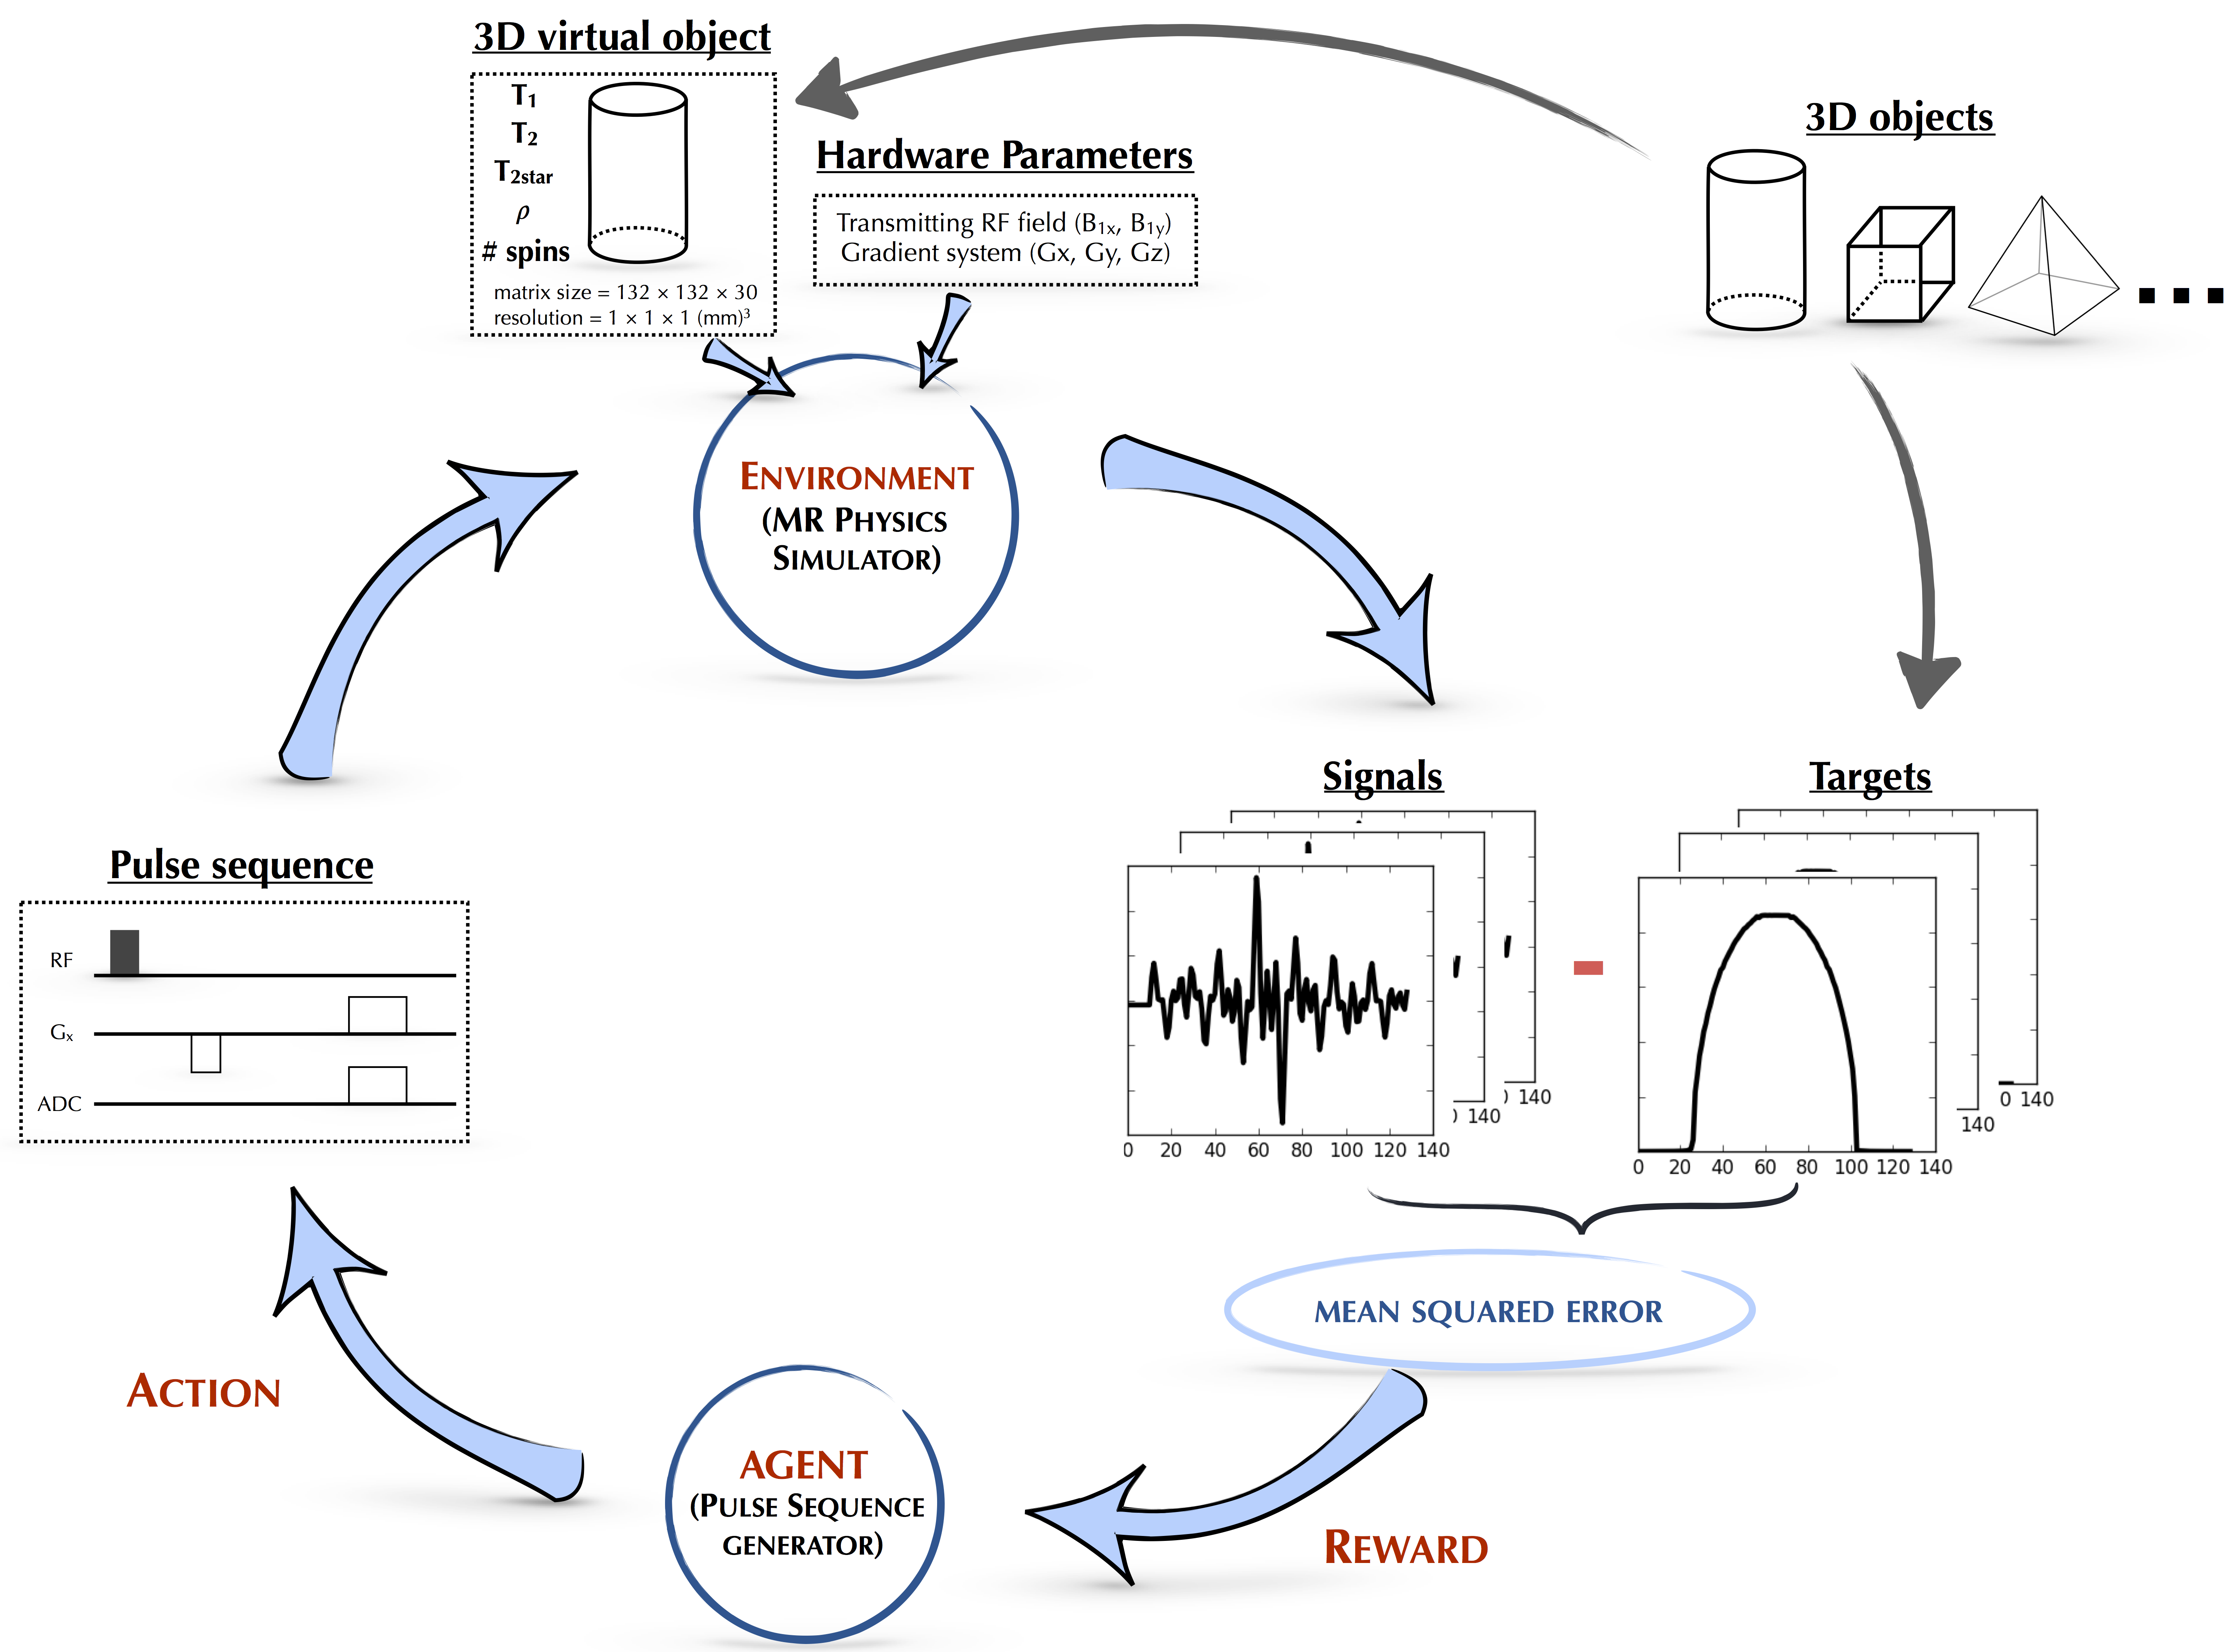
\includegraphics[scale=0.6]{schematic.png}
    \caption{Schematic of the AUTOSEQ Reinforcement Learning framework \citep{0438}.}
    \label{schematic}
\end{figure}